% Created by tikzDevice version 0.12.3.1 on 2022-04-26 16:42:16
% !TEX encoding = UTF-8 Unicode
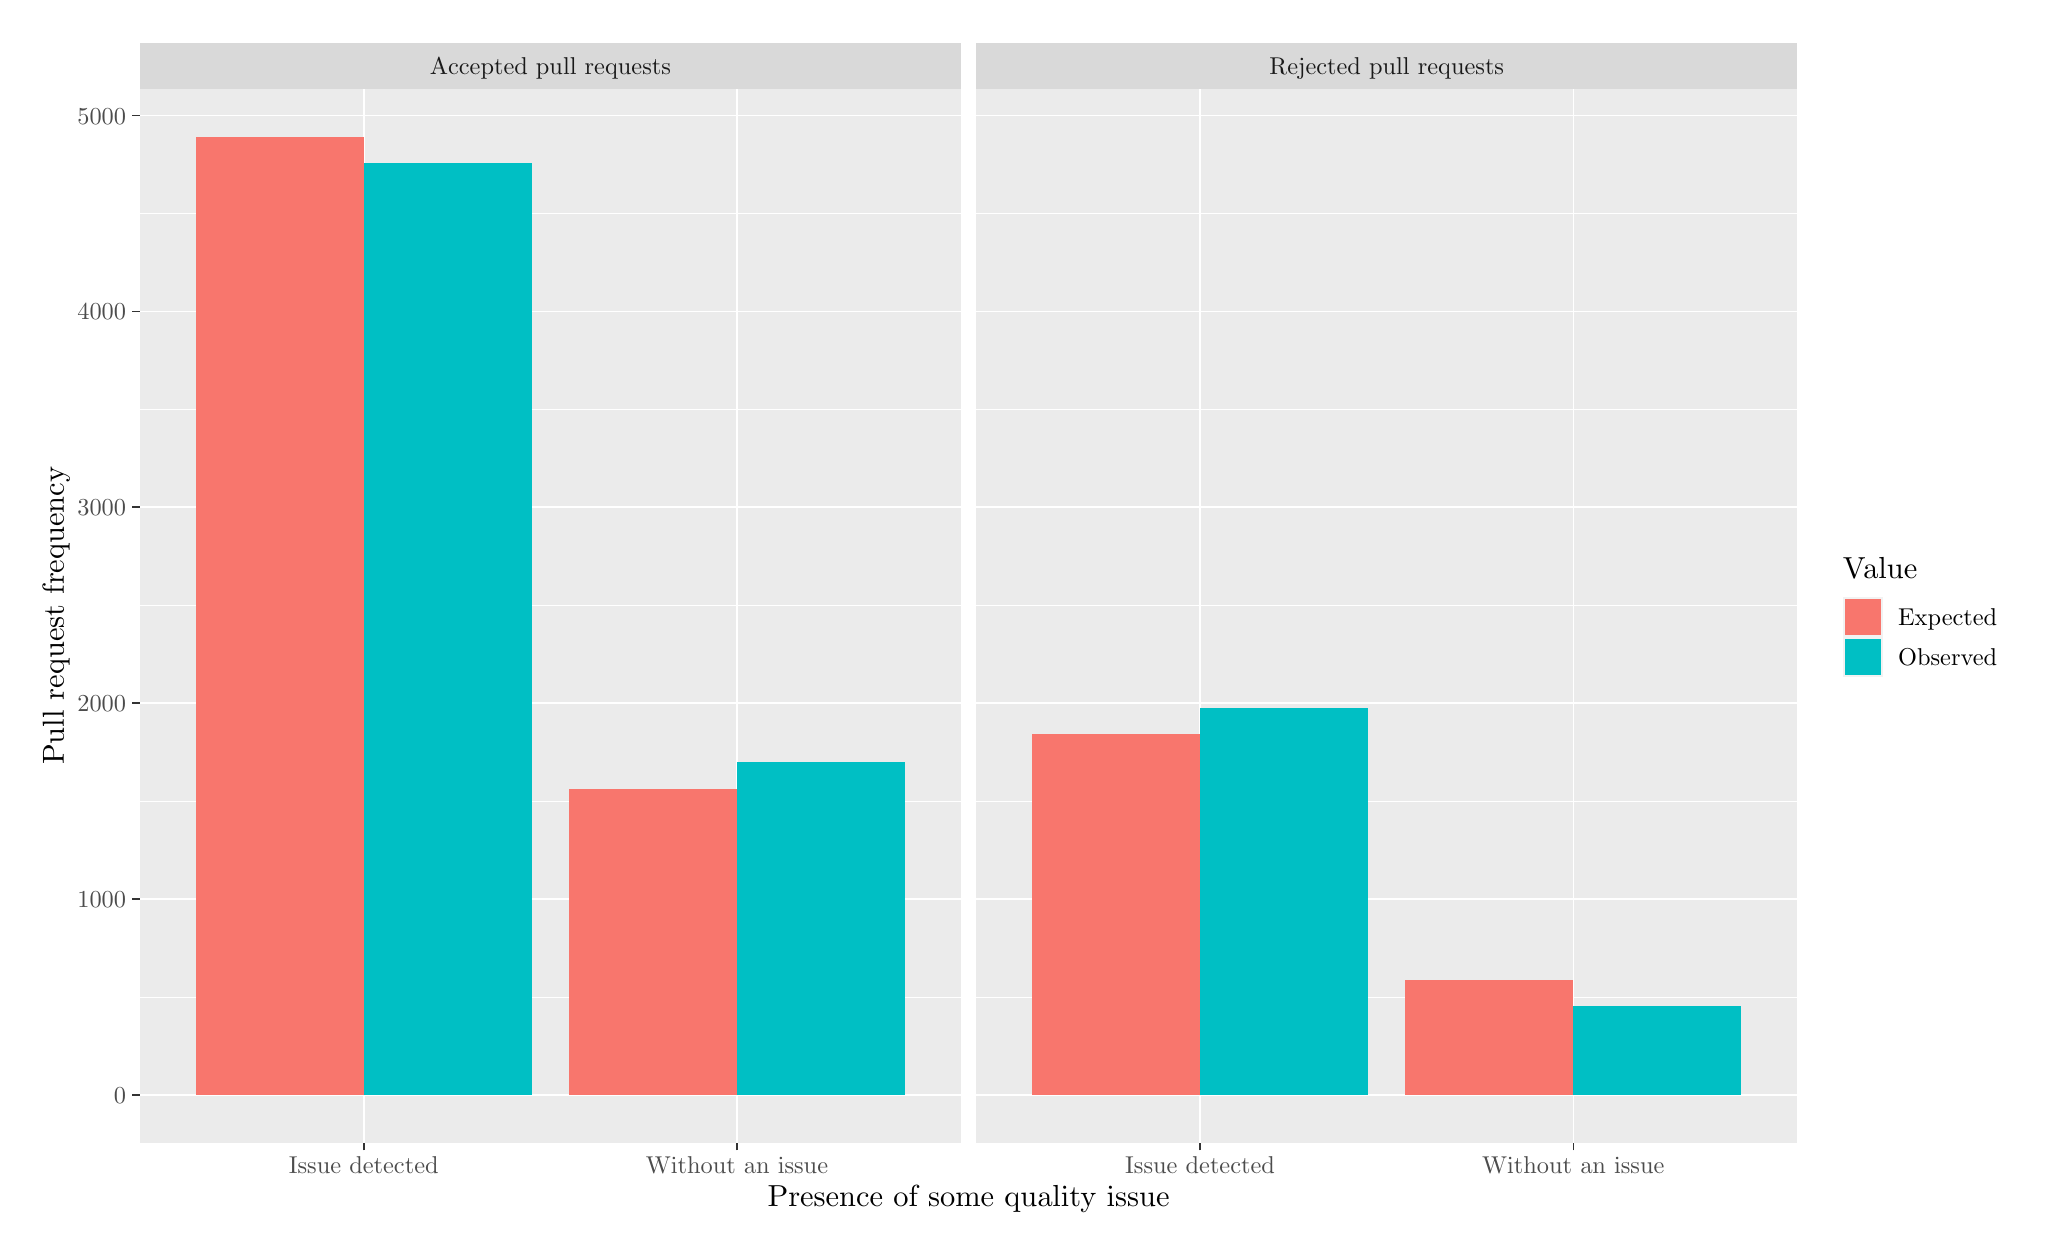
\begin{tikzpicture}[x=1pt,y=1pt]
\definecolor{fillColor}{RGB}{255,255,255}
\path[use as bounding box,fill=fillColor,fill opacity=0.00] (0,0) rectangle (722.70,433.62);
\begin{scope}
\path[clip] (  0.00,  0.00) rectangle (722.70,433.62);
\definecolor{drawColor}{RGB}{255,255,255}
\definecolor{fillColor}{RGB}{255,255,255}

\path[draw=drawColor,line width= 0.6pt,line join=round,line cap=round,fill=fillColor] (  0.00,  0.00) rectangle (722.70,433.62);
\end{scope}
\begin{scope}
\path[clip] ( 40.51, 30.69) rectangle (337.23,411.55);
\definecolor{fillColor}{gray}{0.92}

\path[fill=fillColor] ( 40.51, 30.69) rectangle (337.23,411.55);
\definecolor{drawColor}{RGB}{255,255,255}

\path[draw=drawColor,line width= 0.3pt,line join=round] ( 40.51, 83.38) --
	(337.23, 83.38);

\path[draw=drawColor,line width= 0.3pt,line join=round] ( 40.51,154.15) --
	(337.23,154.15);

\path[draw=drawColor,line width= 0.3pt,line join=round] ( 40.51,224.91) --
	(337.23,224.91);

\path[draw=drawColor,line width= 0.3pt,line join=round] ( 40.51,295.68) --
	(337.23,295.68);

\path[draw=drawColor,line width= 0.3pt,line join=round] ( 40.51,366.45) --
	(337.23,366.45);

\path[draw=drawColor,line width= 0.6pt,line join=round] ( 40.51, 48.00) --
	(337.23, 48.00);

\path[draw=drawColor,line width= 0.6pt,line join=round] ( 40.51,118.76) --
	(337.23,118.76);

\path[draw=drawColor,line width= 0.6pt,line join=round] ( 40.51,189.53) --
	(337.23,189.53);

\path[draw=drawColor,line width= 0.6pt,line join=round] ( 40.51,260.30) --
	(337.23,260.30);

\path[draw=drawColor,line width= 0.6pt,line join=round] ( 40.51,331.07) --
	(337.23,331.07);

\path[draw=drawColor,line width= 0.6pt,line join=round] ( 40.51,401.83) --
	(337.23,401.83);

\path[draw=drawColor,line width= 0.6pt,line join=round] (121.43, 30.69) --
	(121.43,411.55);

\path[draw=drawColor,line width= 0.6pt,line join=round] (256.30, 30.69) --
	(256.30,411.55);
\definecolor{fillColor}{RGB}{0,191,196}

\path[fill=fillColor] (121.43, 48.00) rectangle (182.12,384.71);

\path[fill=fillColor] (256.30, 48.00) rectangle (317.00,168.16);
\definecolor{fillColor}{RGB}{248,118,109}

\path[fill=fillColor] ( 60.74, 48.00) rectangle (121.43,394.24);

\path[fill=fillColor] (195.61, 48.00) rectangle (256.30,158.63);
\end{scope}
\begin{scope}
\path[clip] (342.73, 30.69) rectangle (639.44,411.55);
\definecolor{fillColor}{gray}{0.92}

\path[fill=fillColor] (342.73, 30.69) rectangle (639.44,411.55);
\definecolor{drawColor}{RGB}{255,255,255}

\path[draw=drawColor,line width= 0.3pt,line join=round] (342.73, 83.38) --
	(639.44, 83.38);

\path[draw=drawColor,line width= 0.3pt,line join=round] (342.73,154.15) --
	(639.44,154.15);

\path[draw=drawColor,line width= 0.3pt,line join=round] (342.73,224.91) --
	(639.44,224.91);

\path[draw=drawColor,line width= 0.3pt,line join=round] (342.73,295.68) --
	(639.44,295.68);

\path[draw=drawColor,line width= 0.3pt,line join=round] (342.73,366.45) --
	(639.44,366.45);

\path[draw=drawColor,line width= 0.6pt,line join=round] (342.73, 48.00) --
	(639.44, 48.00);

\path[draw=drawColor,line width= 0.6pt,line join=round] (342.73,118.76) --
	(639.44,118.76);

\path[draw=drawColor,line width= 0.6pt,line join=round] (342.73,189.53) --
	(639.44,189.53);

\path[draw=drawColor,line width= 0.6pt,line join=round] (342.73,260.30) --
	(639.44,260.30);

\path[draw=drawColor,line width= 0.6pt,line join=round] (342.73,331.07) --
	(639.44,331.07);

\path[draw=drawColor,line width= 0.6pt,line join=round] (342.73,401.83) --
	(639.44,401.83);

\path[draw=drawColor,line width= 0.6pt,line join=round] (423.65, 30.69) --
	(423.65,411.55);

\path[draw=drawColor,line width= 0.6pt,line join=round] (558.52, 30.69) --
	(558.52,411.55);
\definecolor{fillColor}{RGB}{0,191,196}

\path[fill=fillColor] (423.65, 48.00) rectangle (484.34,187.90);

\path[fill=fillColor] (558.52, 48.00) rectangle (619.21, 80.13);
\definecolor{fillColor}{RGB}{248,118,109}

\path[fill=fillColor] (362.96, 48.00) rectangle (423.65,178.37);

\path[fill=fillColor] (497.83, 48.00) rectangle (558.52, 89.66);
\end{scope}
\begin{scope}
\path[clip] ( 40.51,411.55) rectangle (337.23,428.12);
\definecolor{fillColor}{gray}{0.85}

\path[fill=fillColor] ( 40.51,411.55) rectangle (337.23,428.12);
\definecolor{drawColor}{gray}{0.10}

\node[text=drawColor,anchor=base,inner sep=0pt, outer sep=0pt, scale=  0.88] at (188.87,416.80) {Accepted pull requests};
\end{scope}
\begin{scope}
\path[clip] (342.73,411.55) rectangle (639.44,428.12);
\definecolor{fillColor}{gray}{0.85}

\path[fill=fillColor] (342.73,411.55) rectangle (639.44,428.12);
\definecolor{drawColor}{gray}{0.10}

\node[text=drawColor,anchor=base,inner sep=0pt, outer sep=0pt, scale=  0.88] at (491.09,416.80) {Rejected pull requests};
\end{scope}
\begin{scope}
\path[clip] (  0.00,  0.00) rectangle (722.70,433.62);
\definecolor{drawColor}{gray}{0.20}

\path[draw=drawColor,line width= 0.6pt,line join=round] (121.43, 27.94) --
	(121.43, 30.69);

\path[draw=drawColor,line width= 0.6pt,line join=round] (256.30, 27.94) --
	(256.30, 30.69);
\end{scope}
\begin{scope}
\path[clip] (  0.00,  0.00) rectangle (722.70,433.62);
\definecolor{drawColor}{gray}{0.30}

\node[text=drawColor,anchor=base,inner sep=0pt, outer sep=0pt, scale=  0.88] at (121.43, 19.68) {Issue detected};

\node[text=drawColor,anchor=base,inner sep=0pt, outer sep=0pt, scale=  0.88] at (256.30, 19.68) {Without an issue};
\end{scope}
\begin{scope}
\path[clip] (  0.00,  0.00) rectangle (722.70,433.62);
\definecolor{drawColor}{gray}{0.20}

\path[draw=drawColor,line width= 0.6pt,line join=round] (423.65, 27.94) --
	(423.65, 30.69);

\path[draw=drawColor,line width= 0.6pt,line join=round] (558.52, 27.94) --
	(558.52, 30.69);
\end{scope}
\begin{scope}
\path[clip] (  0.00,  0.00) rectangle (722.70,433.62);
\definecolor{drawColor}{gray}{0.30}

\node[text=drawColor,anchor=base,inner sep=0pt, outer sep=0pt, scale=  0.88] at (423.65, 19.68) {Issue detected};

\node[text=drawColor,anchor=base,inner sep=0pt, outer sep=0pt, scale=  0.88] at (558.52, 19.68) {Without an issue};
\end{scope}
\begin{scope}
\path[clip] (  0.00,  0.00) rectangle (722.70,433.62);
\definecolor{drawColor}{gray}{0.30}

\node[text=drawColor,anchor=base east,inner sep=0pt, outer sep=0pt, scale=  0.88] at ( 35.56, 44.97) {0};

\node[text=drawColor,anchor=base east,inner sep=0pt, outer sep=0pt, scale=  0.88] at ( 35.56,115.73) {1000};

\node[text=drawColor,anchor=base east,inner sep=0pt, outer sep=0pt, scale=  0.88] at ( 35.56,186.50) {2000};

\node[text=drawColor,anchor=base east,inner sep=0pt, outer sep=0pt, scale=  0.88] at ( 35.56,257.27) {3000};

\node[text=drawColor,anchor=base east,inner sep=0pt, outer sep=0pt, scale=  0.88] at ( 35.56,328.03) {4000};

\node[text=drawColor,anchor=base east,inner sep=0pt, outer sep=0pt, scale=  0.88] at ( 35.56,398.80) {5000};
\end{scope}
\begin{scope}
\path[clip] (  0.00,  0.00) rectangle (722.70,433.62);
\definecolor{drawColor}{gray}{0.20}

\path[draw=drawColor,line width= 0.6pt,line join=round] ( 37.76, 48.00) --
	( 40.51, 48.00);

\path[draw=drawColor,line width= 0.6pt,line join=round] ( 37.76,118.76) --
	( 40.51,118.76);

\path[draw=drawColor,line width= 0.6pt,line join=round] ( 37.76,189.53) --
	( 40.51,189.53);

\path[draw=drawColor,line width= 0.6pt,line join=round] ( 37.76,260.30) --
	( 40.51,260.30);

\path[draw=drawColor,line width= 0.6pt,line join=round] ( 37.76,331.07) --
	( 40.51,331.07);

\path[draw=drawColor,line width= 0.6pt,line join=round] ( 37.76,401.83) --
	( 40.51,401.83);
\end{scope}
\begin{scope}
\path[clip] (  0.00,  0.00) rectangle (722.70,433.62);
\definecolor{drawColor}{RGB}{0,0,0}

\node[text=drawColor,anchor=base,inner sep=0pt, outer sep=0pt, scale=  1.10] at (339.98,  7.64) {Presence of some quality issue};
\end{scope}
\begin{scope}
\path[clip] (  0.00,  0.00) rectangle (722.70,433.62);
\definecolor{drawColor}{RGB}{0,0,0}

\node[text=drawColor,rotate= 90.00,anchor=base,inner sep=0pt, outer sep=0pt, scale=  1.10] at ( 13.08,221.12) {Pull request frequency};
\end{scope}
\begin{scope}
\path[clip] (  0.00,  0.00) rectangle (722.70,433.62);
\definecolor{fillColor}{RGB}{255,255,255}

\path[fill=fillColor] (650.44,193.56) rectangle (717.20,248.68);
\end{scope}
\begin{scope}
\path[clip] (  0.00,  0.00) rectangle (722.70,433.62);
\definecolor{drawColor}{RGB}{0,0,0}

\node[text=drawColor,anchor=base west,inner sep=0pt, outer sep=0pt, scale=  1.10] at (655.94,234.53) {Value};
\end{scope}
\begin{scope}
\path[clip] (  0.00,  0.00) rectangle (722.70,433.62);
\definecolor{fillColor}{gray}{0.95}

\path[fill=fillColor] (655.94,213.51) rectangle (670.40,227.96);
\end{scope}
\begin{scope}
\path[clip] (  0.00,  0.00) rectangle (722.70,433.62);
\definecolor{fillColor}{RGB}{248,118,109}

\path[fill=fillColor] (656.65,214.22) rectangle (669.69,227.25);
\end{scope}
\begin{scope}
\path[clip] (  0.00,  0.00) rectangle (722.70,433.62);
\definecolor{fillColor}{gray}{0.95}

\path[fill=fillColor] (655.94,199.06) rectangle (670.40,213.51);
\end{scope}
\begin{scope}
\path[clip] (  0.00,  0.00) rectangle (722.70,433.62);
\definecolor{fillColor}{RGB}{0,191,196}

\path[fill=fillColor] (656.65,199.77) rectangle (669.69,212.80);
\end{scope}
\begin{scope}
\path[clip] (  0.00,  0.00) rectangle (722.70,433.62);
\definecolor{drawColor}{RGB}{0,0,0}

\node[text=drawColor,anchor=base west,inner sep=0pt, outer sep=0pt, scale=  0.88] at (675.90,217.71) {Expected};
\end{scope}
\begin{scope}
\path[clip] (  0.00,  0.00) rectangle (722.70,433.62);
\definecolor{drawColor}{RGB}{0,0,0}

\node[text=drawColor,anchor=base west,inner sep=0pt, outer sep=0pt, scale=  0.88] at (675.90,203.25) {Observed};
\end{scope}
\end{tikzpicture}
